\chapter{BENZER MİMARİLER VE ÖNCEKİ ÇALIŞMALAR}
Paralel hesaplama için literatürde var olan mimariler Flynn taksonomisi adıyla binilen bir sınıflandırmaya tabidir. Söz konusu donanım, özelliklerine göre bu sınıflandırmada bir sınıfa yerleştirilir. Literatür taramasında öncelikle bu sınıflandırmadan bahsedilmiş, ardından belirlenen sınıfta ön plana çıkan mimariler incelenmiştir.

\section{Paralel işleme taksonomisi}
Bilgisayar bilimlerindeki tüm uygulamalar ve donanımlar paralellik bakımından 4 sınıfta incelenir. Bu sınıflandırma literatürde Flynn Taksonomisi adıyla geçer \cite{flynnTaxonomy}. Literatürdeki kısaltmalarıyla bu 4 sınıf, SISD (Single Instruction Single Data), SIMD (Single Instruction Multiple Data), MISD (Multiple Instruction Single Data) ve MIMD (Multiple Instruction Multiple Data) şeklinde isimlendirilir. 

\begin{figure}
\centering
\shorthandoff{=}
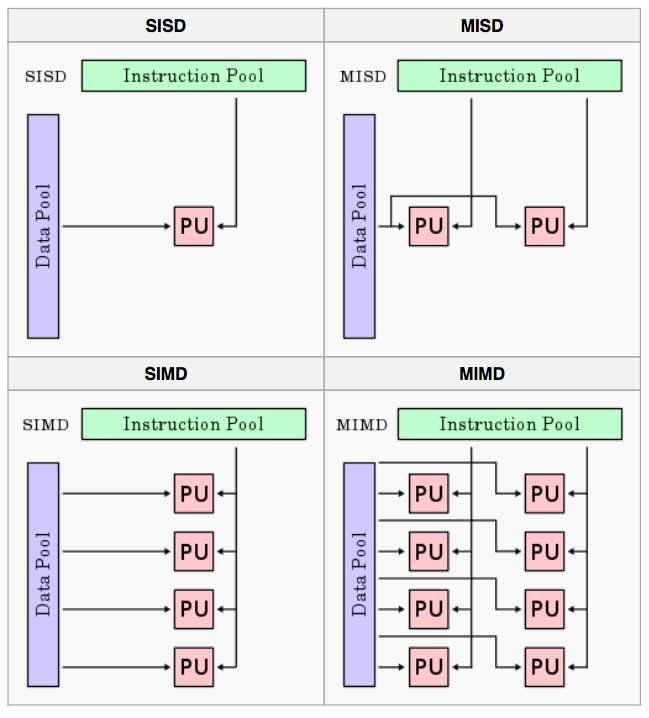
\includegraphics[width=0.9\textwidth]{gorsel/flynnTaxonomy.png}
\shorthandoff{=}
\caption{Flynn Taksonomisi}
\label{overflow}
\end{figure}

SISD mimarilerde herhangi bir paralellikten bahsetmek söz konusu değildir. Tek thread çalıştıran mimariler SISD için örnek olarak gösterilebilir. \par

SIMD mimariler bir buyruğun birden fazla veri seti üzerinde çalıştırıldığı mimarilerdir. Örneğin NxM büyüklüğünde matrislerin toplandığı bir matris toplama işleminde NxM adet veri seti üzerinde basit bir toplama işlemi yapılmaktadır. Gereksinimler ışığında SIMD mimari bu çalışmanın mimari alternatifleri arasındadır. \par

MISD mimariler bir veri seti üzerinde birden fazla buyruğun çalıştırıldığı mimarilerdir. MISD yaygın olarak hata düzelten sistemlerde tercih edilir. Örneğin uzay ortamında çalışması hedeflenen bir hesaplama biriminin ışımalara maruz kalması sebebiyle hesaplamasında veya kaydettiği sonuçlarda yanlışlık olabilir \cite{shivakumar2002modeling}. Bu tarz potansiyel problemlere önlem olarak yapılan her işlem aynı veri seti üzerinde birden fazla kez yapılır ve sonuçlar birden fazla yerde saklanır. Daha sonra aynı verinin kopyaları arasında karşılaştırma yapılırak hatalar algılanır ve düzeltilir. \par

MIMD mimariler bu taksonominin en karmaşık mimarileri olup birden fazla veri seti üzerinde birden fazla buyruğun çalıştırıldığı mimarilerdir. Buna örnek olarak günümüzde kullanılan CPU mimarileri verilebilir. Örneğin Intel Larrabee mimarisi GPU mimarisinde işlevsellik bakımından geliştirilmiş çekirdeklerin kullanılması ile ortaya çıkan bir GPGPU (General Purpose Graphical Processing Unit) olup aynı anda birden fazla veri seti üzerinde birden fazla işlemi koşturabilmektedir \cite{seiler2008larrabee}.\par

Proje gereksinimlerinde ve fonksiyon listesinde belirtilen, hedef donanım hakkındaki ihtiyaçlar, Flynn taksonomisinde SIMD sınıfı ile örtüşmektedir. MIMD bir mimari ise proje gereksinimlerinin üzerinde bir özellik olup, eniyileştirmeye yönelik bir çalışma olabilir.

\section{Mevcut Mimariler}
Gereksinimlerde belirtilen fonksiyonlar ışığında hesaplamalar için kullanılacak modüller belli IPCore donanımları ve basit hesaplama modüllerinden oluşur. Paralel işlemeye özel donanımlarda yürütme zamanının en büyük bileşeni verilerin okunması ve yazılmasından oluşan bellek işlemleri olduğu için mimari seviyesinde donanım özelliklerini belirleyici unsur, veri yolu tasarımıdır.\par

Veri yolu mimarisi, bellek, yazmaç öbekleri ve hesaplama birimleri arasındaki bağlantı ile bu yapıların mimari hiyerarşisinden oluşur. Literatürde öne çıkan veri yolu mimarileri üç sınıfta değerlendirilebilir: Homojen az çekirdekli işlemciler, homojen çok çekirdekli işlemciler ve heterojen yapıdaki işlemciler. \par

\subsection{Homojen az çekirdekli işlemciler}
Homojen az çekirdekli mimariler birbirinin aynı olan az sayıda yüksek işlem kapasiteli çekirdeklerin 2. veya daha üst seviyede önbellekler üzerinden veri paylaşımı sağladığı işlemcilerdir. Bu mimaride her işlemci çekirdeğin kendisine ait bir önbelleği vardır. Bunlar bir interconnect yardımıyla bütünleşik bir paylaşımlı önbelleğe bağlanırlar. Bu yapıya örnek olarak Intel'in Nehalem işlemcisi gösterilebilir \cite{molka2009memory} \cite{hackenberg2009comparing}. Nehalem mimarisinde hususi önbellek 2 seviyeye ayrılmıştır ve paylaşımlı önbellek 3. seviyeyi oluşturmaktadır. Çekirdekler 3. seviye önbelleğin ardından Şekil \ref{image:nehalem}'deki gibi bir bellek denetleyicisi ile sistemin ana belleğine bağlanır.\par

\begin{figure}
\centering
\shorthandoff{=}
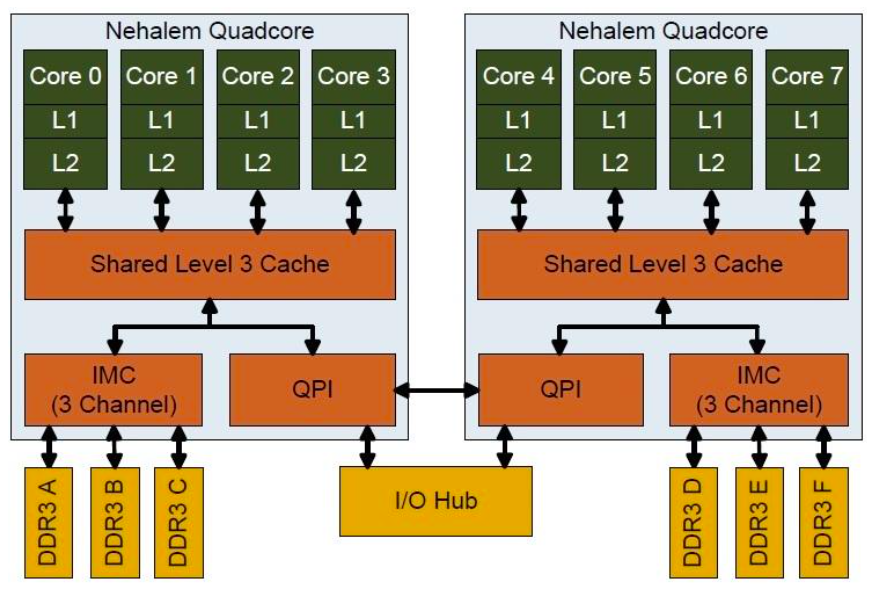
\includegraphics[width=0.9\textwidth]{gorsel/nehalem.jpg}
\shorthandoff{=}
\caption{Intel Nehalem Mimarisi}
\label{image:nehalem}
\end{figure}

\subsection{Homojen çok çekirdekli işlemciler}
Homojen çok çekirdekli mimariler birbirinin aynı olan çok sayıda düşük işlem kapasiteli çekirdeklerden oluşan yapılardır. Bunlara örnek olarak grafik işlemcileri verilebilir \cite{MCSE.2012.23}. Şekil \ref{image:nvidiagpu}'teki gibi bir yapıya sahip olan grafik işlemcilerde amaç, paralelliği ön plana çıkarmak, çok sayıda verinin aynı anda işlenebilmesine olanak sağlamaktır. Az çekirdekli işlemcilerin aksine belleği kullanmak isteyen daha çok çekirdek olacağından bu mimarilerde bellek açısından bir darboğaz oluşmasına sebep olur. Homojen çok çekirdekli mimarilerin bellek hiyerarşisi 2 seviyeli önbellek ve ana bellekten oluşur. Her iki önbellek de çekirdek adacığında paylaşımlıdır. Az çekirdekli mimarilerin aksine çok çekirdekli mimarilerde genel bir yazmaç öbeği tüm çekirdeklerin erişimine açık olup yürütme zamanında her bir çekirdeğe özel olarak atanır.

%\begin{figure}[h] \label{image:nvidiagpu} 
%\centering 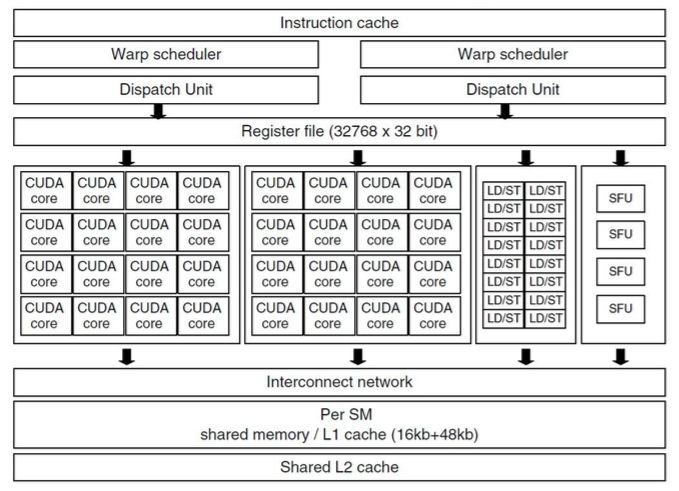
\includegraphics[width=300pt]{gorsel/nvidiagpu.jpg} \caption{Nvidia GPU}  
%\end{figure}

\begin{figure}
\centering
\shorthandoff{=}
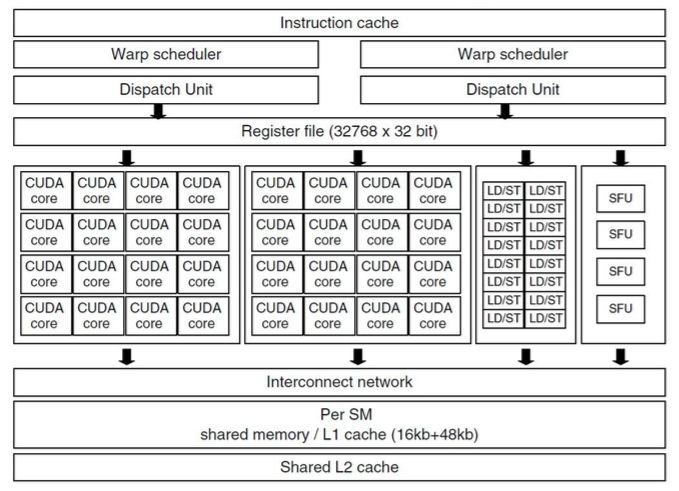
\includegraphics[width=0.9\textwidth]{gorsel/nvidiagpu.jpg}
\shorthandoff{=}
\caption{Nvidia GPU}
\label{image:nvidiagpu}
\end{figure}



Homojen az çekirdekli mimariler genel amaçlı kullanılan CPU (Central Processing Unit) mimarilerinde tercih edilirken çok çekirdekli mimariler GPU (Graphical Processing Unit) ön plana çıkar. CPU çekirdekleri yüksek işlem gücüne sahip ve az sayıda iken GPU çekirdekleri düşük işlem gücüne sahip ve çok sayıdadır. CPU üzerinde koşturulan programların dallanma ve bellek işlemleri için harcadığı zamanın azaltılması için çekirdeklere yakın büyük kapasiteli önbellekler kullanılır. GPU çekirdeklerinin sayıca fazla olması paralel hesaplamayı ön plana çıkarmakta ve ana bellek erişimi için kullanılan veri yolu genişliği, önbellek büyüklüğünden daha önemli bir kriter olmaktadır. Tablo \ref{table:cpuGpuComparision} içinde CPU ve GPU mimarilerinin bellek özellikleri sunulmuştur \cite{cpuGpuMemoryTable}. \par

\begin{longtable}{p{150pt} p{100pt} p{100pt}}
\caption[CPU GPU Bellek Karşılaştırması]{CPU GPU Bellek Karşılaştırması} \label{table:cpuGpuComparision} \\
\multicolumn{1}{c}{} & \multicolumn{1}{c}{\textbf{CPU}} & \multicolumn{1}{c}{\textbf{GPU}} \\ 
\hline 
\endfirsthead

\multicolumn{2}{c}%
{{\bfseries \tablename\ \thetable{} -- devam}} \\
\multicolumn{1}{c}{} & \multicolumn{1}{c}{\textbf{CPU}} & \multicolumn{1}{c}{\textbf{GPU}} \\  
\hline 
\endhead

\hline 
\multicolumn{3}{r}{{Sonraki sayfada devam etmektedir.}} \\ 
\endfoot

\hline \hline
\endlastfoot
  Bellek 									&		 6 -  64 GB 		& 	768 MB - 6 GB 	\\
  Bellek Bant Genişliği 	&		24 -  32 GB/s 	& 	100 - 200 GB/s 	\\
  L2 Önbellek				 			&		 8 -  15 MB 		& 	512 - 768 KB 		\\
  L1 Önbellek				 			&	 256 - 512 KB 		& 	 16 -  48 KB 		\\
\end{longtable}

Homojen çok çekirdekli mimarilere verilebilecek bir örnek de sunucu sistemlerinde kullanılan Tile mimarisidir. \cite{tileArchitecture} Bu mimaride 36-100 arasında RISC işlemciden oluşan çekirdekler birbirlerine bağlanarak yüksek paralellik elde edilir. Tile mimarisinde bellek mimarisi olarak şekil  \ref{image:tileArchitecture}'te sunulan NUCA (non-uniform cache architecture) önbellek mimarisi kullanılır. Bu mimaride çekirdeklerin her birinin kendine ait özel önbelleği vardır. İkinci seviye önbellek olarak diğer çekirdeklerin önbellekleri kullanılır. Örnek olarak, 64 çekirdekli bir işlemcide her bir çekirdeğin 32 KB önbelleği olduğunu varsayarsak; 1 numaralı çekirdeğin 32 KB 1. seviye ve 2016 KB 2. seviye önbelleği olacaktır. Bu tasarımda herhangi bir çekirdeğin diğer tüm çekirdeklerin önbelleklerine bağlantısı olmalıdır. Çekirdek sayısının artması ile bu gereksinim bir wiring problemine dönüşür ve uzun yollar kritik yolu etkileyerek toplam gecikmeye katkıda bulunabilir. Bu kısıttan dolayı Tile mimarisinde 2 boyutlu bir MESH ağı kurulmuş ve her bir çekirdek bu ağdaki bir node olarak yerleştirilmiştir. Her node bir çekirdek, bir önbellek ve bir routerdan oluşur. Bir çekirdek kendinden farklı tüm çekirdeklerin ön belleklerini ikinci seviye ön bellek olarak kullandığından MESH network üzerinden her birine erişimi vardır. Ancak fiziksel olarak kendisine uzak olan veriye erişebilmesi komşuluğundaki routerlar üzerinden her seferinde bir birim şeklindedir. Bu davranış satranç tahtası üzerinde şahın hareketi gibi düşünülebilir. MESH network yapısında tüm verilere erişim hızı aynı olmamakla birlikte, maksimum gecikme, node sayısının karekökü ile orantılı olarak artar. 

\begin{figure}
\centering
\shorthandoff{=}
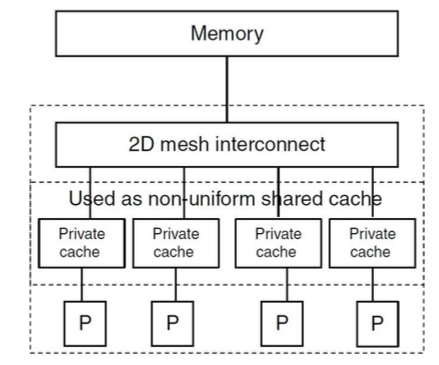
\includegraphics[width=0.9\textwidth]{gorsel/tileArchitecture.png}
\shorthandoff{=}
\caption{Tile Mimarisi}
\label{image:tileArchitecture}
\end{figure}

\subsection{Heterojen yapıdaki işlemciler}
Birbirinin aynı olan çekirdeklerin az veya çok sayıda gerçeklenmesi ile elde edilen paralel hesaplama donanımları çoğu uygulamada performans açısından yeterli gelse de, bir takım uygulamalarda sık kullanılan bazı işlemlerin hızlandırılması adına özel donanımlar gerçeklenir. Literatürde bu tip işlemciler heterojen yapıdaki işlemciler olarak adlandırılır. Heterojen mimariler doğrudan amaca yönelik hazırlandıkları için çok farklı mimari yapılarda gerçeklenebilirler. Heterojen mimarilerin temel özelliği bir işi her zaman o işi en hızlı yapan donanıma vermeleridir. Bu sebeple sık kullanılan hemen her işlem için ayrı hesaplama birimleri yerleştirilerek, özel fonksiyonların yazılım seviyesinden donanım seviyesine indirilmesi sağlanır. Örnek olarak şekil \ref{image:playStationArchitecture}'te sunulan heterojen mimari çizimi Playstation oyun konsollarında kullanılan Cell mimarisine aittir. 


\begin{figure}
\centering
\shorthandoff{=}
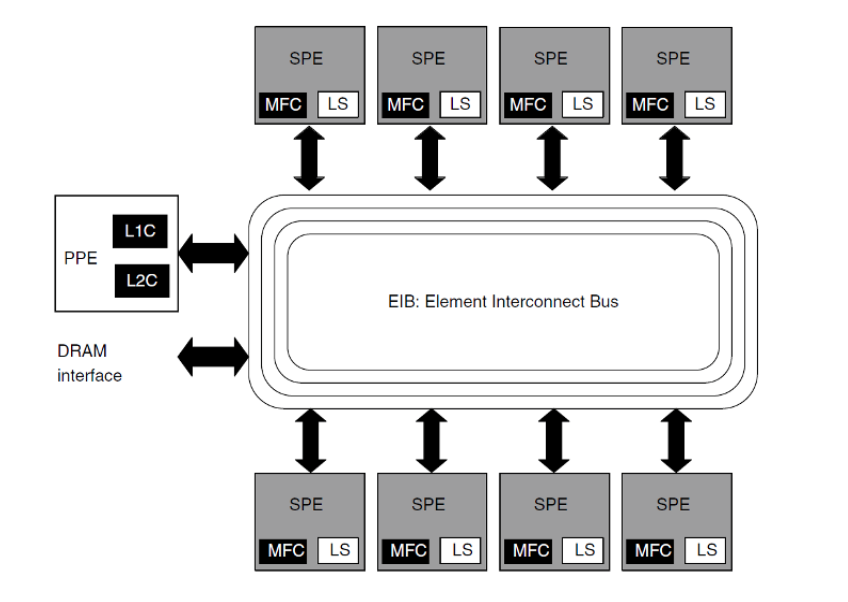
\includegraphics[width=0.9\textwidth]{gorsel/playStationArchitecture.png}
\shorthandoff{=}
\caption{Sony Playstation Cell Mimarisi}
\label{image:playStationArchitecture}
\end{figure}


Şekil \ref{image:playStationArchitecture}'te gösterilen Cell mimarisinde PPE (Power processing element) ana işlemci olup, SPE (Synergistic processing element) bloklarının her biri ise DSP benzeri SIMD işlemcilerdir.